% %%%%%%%%%%%%%%%%%%%%%%%%%%%%%%%%%%%%%%%%%%%%%%%%%%%%%%%%%%%%%%%%%%%%%%%%%%%%%
% thesis.tex: Primary TeX control file for thesis.
% %%%%%%%%%%%%%%%%%%%%%%%%%%%%%%%%%%%%%%%%%%%%%%%%%%%%%%%%%%%%%%%%%%%%%%%%%%%%%
\documentclass[11pt, oneside]{mnthesis}
\usepackage{epsfig} % Allows the inclusion of eps files
\usepackage{epic} % Enhanced picture mode
\usepackage{eepic} % Extensions for epic
\usepackage{units} % SI unit typesetting
\usepackage{url} % URL handling
\usepackage{longtable} % Tables that continue onto multiple pages
\usepackage{mathrsfs} % Support for \mathscr script
\usepackage{multirow} % Span rows in tables
\usepackage{bigstrut} % Space struts in tables up and down
\usepackage{amssymb} % AMS math symbols and helpers
\usepackage{graphicx} % Enhanced graphics support
\usepackage{setspace} % Adjust spacing in captions, single by default
\usepackage{xspace} % Automatically adjusting space after macros
\usepackage{amsmath} % \text, and other math formatting options
\usepackage{siunitx} % \num{} formatting and SI unit formatting
\usepackage{booktabs} % Enhanced tables with \toprule, etc.
\usepackage{hyperref} % Add clickable links to other parts of the document
\usepackage[noabbrev]{cleveref} % Automatically determine \cref type

% Configure the siunitx package
\sisetup{
    group-separator = {,}, % Use , to separate groups of digits, like 12,345
    list-final-separator = {, and } % Always use the serial comma in \SIlist
}

% Configure the cleveref package
\newcommand{\creflastconjunction}{, and } % Always use the serial comma




% Names with special characters. 
\newcommand{\Alfven}{Alfv\'en\xspace}
\newcommand{\Ampere}{Amp\`ere\xspace}

% To make sure the capitalization is consistent. 
\newcommand{\ohmlaw}{Ohm's Law\xspace}
\newcommand{\amplaw}{\Ampere's Law\xspace}
\newcommand{\farlaw}{Faraday's Law\xspace}

% Field-aligned unit vectors. 
\newcommand{\xhat}{\ensuremath{\hat{x}}\xspace}
\newcommand{\yhat}{\ensuremath{\hat{y}}\xspace}
\newcommand{\zhat}{\ensuremath{\hat{z}}\xspace}

% Spherical unit vectors. 
\newcommand{\rhat}{\ensuremath{\hat{r}}\xspace}
\newcommand{\qhat}{\ensuremath{\hat{\theta}}\xspace}
\newcommand{\fhat}{\ensuremath{\hat{\phi}}\xspace}

% Use underlines for vectors and tensors. 
\renewcommand{\vec}[1]{\underline{#1}}
\newcommand{\tensor}[1]{\underline{\underline{#1}}}

% Differential operators. 
\newcommand{\dd}[1]{\ensuremath{ \frac{\partial}{\partial #1} }\xspace}
\newcommand{\ddt}{\dd{t}\xspace}
\newcommand{\curl}[1]{\ensuremath{ \nabla \times \vec{#1} }\xspace}
\renewcommand{\div}[1]{\ensuremath{ \nabla \cdot \vec{#1} }\xspace}
\newcommand{\grad}[1]{\ensuremath{ \nabla #1 }\xspace}

% Properly-scaled parentheses for grouping terms or for arguments. 
\newcommand{\lr}[1]{ \left( #1 \right) }
\newcommand{\lrsmall}[1]{ \left( {\scriptstyle #1} \right) }
\renewcommand{\arg}[1]{\!\lr{#1}}
\newcommand{\argsmall}[1]{\!\lrsmall{#1}}
\newcommand{\lrb}[1]{ \left[ #1 \right] }

% Circled plus-minus symbol. Solving quartics requires \pm and \opm. 
\newcommand{\opm}{ \text{ \textcircled{ \ensuremath{\hskip -0.2em \pm} } } \xspace}

% Define a better looking eV by moving the V slightly left
\DeclareSIUnit\electronvolt{e\hspace{-0.08em}V}

\DeclareSIUnit\RE{R_E}


\newcommand{\dt}{\ensuremath{\delta \hspace{-0.1em} t} \xspace}



% Azimuthal modenumber, typically indicated with a lowercase m. 
\newcommand{\azm}{\ensuremath{m_{azimuthal}}\xspace}

% Azimuthal modenumber, typically indicated with a lowercase m. 
\newcommand{\me}{\ensuremath{m_{e}}\xspace}

% Jacobian dererminant, typically indicated with a capital J, which we are using for current. 
\newcommand{\jac}{\ensuremath{D}\xspace}

% Dispersion tensor, typically indicated with... a capital D?
\newcommand{\dispersiontensor}{\tensor{T}\xspace}


% These things just get used a lot in the dispersion relation chapter...

% Boris-corrected speed of light. 
\newcommand{\cb}{\ensuremath{c_B} \xspace}

% Boris-corrected plasma frequency. 
\newcommand{\ob}{\ensuremath{\omega_B} \xspace}

% Boris-corrected electric constant. 
\newcommand{\eb}{\ensuremath{\epsilon_B} \xspace}

% Alfven speed. 
\newcommand{\va}{\ensuremath{v_A} \xspace}

% Perpendicular electric constant. 
\newcommand{\ep}{\ensuremath{\epsilon_\bot} \xspace}

% Epsilon zero. 
\newcommand{\ez}{\ensuremath{\epsilon_0} \xspace}

% Conductivities. 
\newcommand{\sz}{\ensuremath{\sigma_0} \xspace}
\newcommand{\sh}{\ensuremath{\sigma_H} \xspace}
\renewcommand{\sp}{\ensuremath{\sigma_P} \xspace}




\newcommand{\spe}{\ensuremath{\frac{\sigma_P}{\ep}} \xspace}
\newcommand{\she}{\ensuremath{\frac{\sigma_H}{\ep}} \xspace}




% 3x3 matrix. 
\newcommand{\mmm}[9]{ \left[ \begin{array}{ccc}
    #1 & #2 & #3 \\
    #4 & #5 & #6 \\
    #7 & #8 & #9
  \end{array} \right] }

% 2x2 matrix. 
\newcommand{\mm}[4]{ \left[ \begin{array}{cc}
    #1 & #2 \\
    #3 & #4
  \end{array} \right] }

% 2x1 matrix, or 2-vector. 
\newcommand{\vv}[2]{ \left[ \begin{array}{c}
    #1 \\
    #2
  \end{array} \right] }


% Physics constants
\newcommand{\C}{{\mathrm{c}}}

% Add space between rows of tables
\newcommand{\spacerows}[1]{\renewcommand{\arraystretch}{#1}}









\linespread{1.3}

% Compile only the chapters listed here
\includeonly{
    preliminaries/title,
    chapters/science,
    chapters/waves,
    chapters/model,
    chapters/results,
    chapters/data,
    chapters/conclusion,
    chapters/app_geometry,
    chapters/app_integrating,
}



% %%%%%%%%%%%%%%%%%%%%%%%%%%%%%%%%%%%%%%%%%%%%%%%%%%%%%%%%%%%%%%%%%%%%%%%%%%%%%
% %%%%%%%%%%%%%%%%%%%%%%%%%%%%%%%%%%%%%%%%%%%%%%%%%%%%%%%% Mark this as a draft. 
% %%%%%%%%%%%%%%%%%%%%%%%%%%%%%%%%%%%%%%%%%%%%%%%%%%%%%%%%%%%%%%%%%%%%%%%%%%%%%
\draft






\begin{document}
\bibliographystyle{hunsrt} % style of bibliography

% Title and other sections that come before the body of the document
%%%%%%%%%%%%%%%%%%%%%%%%%%%%%%%%%%%%%%%%%%%%%%%%%%%%%%%%%%%%%%%%%%%%%%%%%%%%%%%%
% title.tex - Set up the beginning of thesis.
%%%%%%%%%%%%%%%%%%%%%%%%%%%%%%%%%%%%%%%%%%%%%%%%%%%%%%%%%%%%%%%%%%%%%%%%%%%%%%%%

% Uncomment to turn on draft mode, which changes the title page to have a draft
% label and date of compilation
%\draft

% Set the type of thesis
\phd % use if for a Ph.D. dissertation
%\ms % use if for a Master of Science thesis

% Set the title and your name. Remember that the guidelines state:
%
% "The title of the thesis must not contain chemical or mathematical formulas,
% symbols, superscripts, subscripts, Greek letters, or other non-standard
% characters; words must be substituted."
\title{\bf Modeling Current-Driven Pc4 Pulsations in Two and a Half Dimensions}
\author{Charles A McEachern}
% Advisor name, put co-advisors here as well separated by commas
\director{Robert L Lysak}

% Specify the month and year; if commented out then these default to the
% current month and year
\submissionmonth{April}
\submissionyear{2016}

% Pages after the title page
\abstract{% %%%%%%%%%%%%%%%%%%%%%%%%%%%%%%%%%%%%%%%%%%%%%%%%%%%%%%%%%%%%%%%%%%%%%%%%%%%%%
% %%%%%%%%%%%%%%%%%%%%%%%%%%%%%%%%%%%%%%%%%%%%%%%%%%%%%%%%%%%%%%%%%%%% Abstract
% %%%%%%%%%%%%%%%%%%%%%%%%%%%%%%%%%%%%%%%%%%%%%%%%%%%%%%%%%%%%%%%%%%%%%%%%%%%%%

Abstract placeholder. 
}
\copyrightpage % Do you want copyright protection?
\acknowledgements{%%%%%%%%%%%%%%%%%%%%%%%%%%%%%%%%%%%%%%%%%%%%%%%%%%%%%%%%%%%%%%%%%%%%%%%%%%%%%%%%
% acknowledge.tex: Acknowledgements
%%%%%%%%%%%%%%%%%%%%%%%%%%%%%%%%%%%%%%%%%%%%%%%%%%%%%%%%%%%%%%%%%%%%%%%%%%%%%%%%

There are many people that have earned my gratitude for their contribution to my
time in graduate school.

%%%%%%%%%%%%%%%%%%%%%%%%%%%%%%%%%%%%%%%%%%%%%%%%%%%%%%%%%%%%%%%%%%%%%%%%%%%%%%%%
}
\dedication{% %%%%%%%%%%%%%%%%%%%%%%%%%%%%%%%%%%%%%%%%%%%%%%%%%%%%%%%%%%%%%%%%%%%%%%%%%%%%%
% %%%%%%%%%%%%%%%%%%%%%%%%%%%%%%%%%%%%%%%%%%%%%%%%%%%%%%%%%%%%%%%%%% Dedication
% %%%%%%%%%%%%%%%%%%%%%%%%%%%%%%%%%%%%%%%%%%%%%%%%%%%%%%%%%%%%%%%%%%%%%%%%%%%%%

\todo{$\cdots$}

}

% Use a special preface
%\extra{\input{preface}}

% The \beforepreface command actually causes insertion of the title,
% abstract, signature, and copyright pages into the new document.
\beforepreface

% Define the text to go before the table of contents
\figurespage
\tablespage

% The \afterpreface command actually causes insertion of the
% contents, list of figures, etc. into the new document.
\afterpreface
%%%%%%%%%%%%%%%%%%%%%%%%%%%%%%%%%%%%%%%%%%%%%%%%%%%%%%%%%%%%%%%%%%%%%%%%%%%%%%%%


% %%%%%%%%%%%%%%%%%%%%%%%%%%%%%%%%%%%%%%%%%%%%%%%%%%%%%%%%%%%%%%%%%%%%%%%%%%%%%
% %%%%%%%%%%%%%%%%%%%%%%%%%%%%%%%%%%%%%%%% Survey of the Near-Earth Environment
% %%%%%%%%%%%%%%%%%%%%%%%%%%%%%%%%%%%%%%%%%%%%%%%%%%%%%%%%%%%%%%%%%%%%%%%%%%%%%

\chapter{From the Sun to the Earth}
\label{science_chapter}


It's all about energy transfer! 

% -----------------------------------------------------------------------------
% -----------------------------------------------------------------------------
% -----------------------------------------------------------------------------
\section{The Solar Core}

% -----------------------------------------------------------------------------
% -----------------------------------------------------------------------------
% -----------------------------------------------------------------------------
\section{The Solar Wind}

% -----------------------------------------------------------------------------
% -----------------------------------------------------------------------------
% -----------------------------------------------------------------------------
\section{Magnetopause and Magnetotail}

% -----------------------------------------------------------------------------
% -----------------------------------------------------------------------------
% -----------------------------------------------------------------------------
\section{Inner Magnetosphere}

Characteristic profiles for $\omega_P$, $\Omega$, $v_A$, $\sigma$, $\epsilon$...


% -----------------------------------------------------------------------------
% -----------------------------------------------------------------------------
% -----------------------------------------------------------------------------
\section{Neutral Atmosphere}




% %%%%%%%%%%%%%%%%%%%%%%%%%%%%%%%%%%%%%%%%%%%%%%%%%%%%%%%%%%%%%%%%%%%%%%%%%%%%%
% %%%%%%%%%%%%%%%%%%%%%%%%%%%%%%%%%%%%%%%%%%%%%% Introduction to Pc4 Pulsations
% %%%%%%%%%%%%%%%%%%%%%%%%%%%%%%%%%%%%%%%%%%%%%%%%%%%%%%%%%%%%%%%%%%%%%%%%%%%%%

\chapter{Ultra Low Frequency Waves}
  \label{ch_waves}




% %%%%%%%%%%%%%%%%%%%%%%%%%%%%%%%%%%%%%%%%%%%%%%%%%%%%%%%%%%%%%%%%%%%%%%%%%%%%%
% %%%%%%%%%%%%%%%%%%%%%%%%%%%%%%%%%%%%%%%%%%%%%% Description of Numerical Model
% %%%%%%%%%%%%%%%%%%%%%%%%%%%%%%%%%%%%%%%%%%%%%%%%%%%%%%%%%%%%%%%%%%%%%%%%%%%%%

\chapter{Numerical Model}
\label{ch_model}

The model works in two and a half dimensions. A meridional slice of the magnetosphere is resolved. Fields are presumed to vary azimuthally according to a fixed modenumber \azm. Derivatives in $\phi$ are replaced by $i \azm$. Imaginary field values indicate a phase shift in the azimuthal direction. 

\todo{Note that Lysak's 2013 paper\cite{lysak_2013} was 2.5D. }

The use of a fixed modenumber allows a dramatic decrease in computational cost. Waves with very high azimuthal modenumber are prohibitively expensive to simulate since they can only be resolved if grid resolution is very fine in the azimuthal direction. 

\todo{Has anyone actually talked about computational expense as a constraint on high-\azm simulations?}

This prevents the simultaneous consideration of dayside and nightside phenomena, but is fine for azimuthally-localized waves. As was shown by \cite{engebretson_1987}, and recently confirmed in detail by \cite{dai_2015}, Pc4 pulsations are generally confined to just a few hours MLT on the dayside. 

Driving with a compressional pulse from the outer boundary of a simulation is typical. This model also includes a novel driving mechanism: perturbations to the ring current. 

The code is linear. All magnetic fields are a first-order perturbation over the zeroth-order dipole field. This is a not-great assumption out towards the magnetopause. In practice, however, most activity is within $L \sim \SI{7}{\RE}$, where the dipole approximation is pretty good. 

Models with height-resolved ionospheres are a very recent development. Lysak presented his in 2013\cite{lysak_2013}. 

Ground signatures are fairly recent as well. 

\todo{Some ground signature work as far back as Greifinger and Greifinger in 1968, but there's been steady advancement. Lysak and Song, in 2006, were the first to work out ground signatures without the assumption of a single-frequency wave. }

\todo{The support software -- the driver and the plotter -- are significant too. Do they go in a section? In an appendix? }

\todo{Past FLR simulations focused on a single mode, didn't account well for the ionosphere, etc. Lee and Lysak 1989, 1990, 1991, Rankin et al 1993, 1995, 1999, Tikhonchuk and Rankin 2000, 2002. }

\todo{Past work that got ground signatures (without latitude-dependent zenith angle) Greifinger and Greifinger 1968, 1973, Hughes 1974, Sciffer and Waters 2002, Sciffer et al 2005. Better computation of ground signatures... Waters and Sciffer 2008, Sciffer and Waters 2011, Woodroffe and Lysak 2012. }

Note that the model uses \si{\mega\meter}, \si{\second}, \si{\mega\coulomb}, and \si{\gram} as the fundamental units of length, time, charge, and mass respectively. As a result, electric field is measured in \si{\mV/\meter}, magnetic field is measured in \si{\nano\tesla}, and Poynting flux is measured in \si{\mW/\meter\squared}. 



% =============================================================================
% =============================================================================
% =============================================================================
\section{Coordinate System}
  \label{sec_coords}

When referring to fields in place, it's convenient to use lowercase\footnote{ Not to be confused with uppercase \X, \Y, and \Z, which orient relative to the sun; see \cref{ch_intro} } \x, \y, and \z in their usual dipolar sense. The unit vector \zhat is aligned with the dipole field (pointing outward in the northern hemisphere and inward in the southern hemisphere), while \xhat is perpendicular to \zhat within the meridional plane and \yhat points in the azimuthal direction. 

\todo{Double-check the signs for \x (radially inward or outward at the equator?) and \y (east or west?). }

\todo{Wait... are \x, \y, and \z the same as Radoski's coordinates? }

It's convenient to align the grid with the zeroth-order magnetic field, which is presumed to be a perfect dipole. Field line resonances (such as Pc4 pulsations) are guided by magnetic field lines. 

\todo{Who showed that ULF waves can be guided? Cite them. }

A typical outermost field line has an equatorial radius of \SI{10}{\RE}. At this point, the ideal dipole approximation is suspect, particularly on the dayside. In practice, however, most wave activity is concentrated around $L \sim \num{7}$. 

\todo{Discuss, in Future Work, how the grid would be generalized. }

Radoski did theoretical work in the following dipole coordinates\cite{radoski_1967_coords}. 
\begin{align}
  \label{radoski_coords}
  \radx & = -\frac{\sin^2 \theta}{r} & \rady & = \phi & \radz & = \frac{\cos \theta}{r^2}
\end{align}

\todo{The symbol $\nu$ is overused. Reserve it for collision frequency. Use something else here. }

It's also convenient to take into account the effects of the ionosphere, the lower boundary of which is governed by gravity, and thus has a more-or-less constant altitude. If the above coordinates are used, no line of constant $\radz$ coincides with the ionosphere, at least not over a significant range of latitudes. 

Many previous works have used an effective ionosphere of nonuniform altitude. 

\todo{Figure out which previous works are worth citing here. Options include Radoski 1967, Lee and Lysak 1989, 1991, Rankin et al 1993, 1994, Streltsov and Lotko 1995, 1999. }


\todo{"The ionosphere is important for \Alfven waves." Cite this. }

In order to accommodate dipole field lines as well as a fixed-altitude ionosphere, a nonorthogonal grid is necessary. Such a grid was worked out numerically by Proehl\cite{proehl_2002}, then formalized analytically by Lysak\cite{lysak_2004}:
\begin{align}
  \label{def_coords}
  \lysakx & = - \frac{R_I}{r} \sin^2 \theta & 
  \lysaky & = \phi &
  \lysakz & = \frac{R_I^2}{r^2} \frac{\cos \theta}{\cos \theta_0}
\end{align}

The term $R_I$ indicates the ionosphere's position relative to Earth's center. It's generally taken to be \SI{1}{\RE} + \SI{100}{\km}. 

Like \radx and \rady, the coordinates \lysakx and \lysaky index a field line. However, compared to \radz, \lysakz has been renormalized by $\cos \theta_0$, where $\theta_0$ is the colatitude where each field line intersects the ionosphere in the northern hemisphere. As a result, for all field lines, $\lysakz = \pm 1$ at the northern and southern foot points. 

In terms of the McIlwain parameter, $\lysakx = -\frac{R_I}{L}$, and $\cos \theta_0 = \sqrt{ 1 - \frac{R_I}{L} }$

Compared to \cref{radoski_coords}, \cref{def_coords} represents a renormalization of indexing along each field line. The field lines themselves are not deformed. 

\todo{Explain how we set up the grid. It should only take a paragraph or two -- it doesn't need its own section. }

\todo{Plot of the grid setup! }

% -----------------------------------------------------------------------------
% -----------------------------------------------------------------------------
% -----------------------------------------------------------------------------
\subsection{Covariant and Contravariant Bases}
  \label{sec_basis}

The coordinates defined in \cref{def_coords} are not orthonormal. As a result, it's necessary to consider covariant and contravariant basis vectors separately. 

Covariant basis vectors $e_i \equiv \dd{\lysaki} \vec{x}$ are normal to the curve defined by constant $\lysaki$. 

Contravariant basis vectors $e^i \equiv \dd{ \vec{x} } \lysaki$ are tangent to the coordinate curve. Equally, they're normal to the plane defined by constant $\lysakj$ for all $j \ne i$. 

The basis vectors are reciprocal to one another\cite{dhaeseleer_1991}, and can be used to define the metric tensor $g$. 
\begin{align}
  \label{metric_basics}
  \hat{e}^i \cdot \hat{e}_j &= \delta^i_j & \hat{e}_i \cdot \hat{e}_j &= g_{ij} & \hat{e}^i \cdot \hat{e}^j &= g^{ij}
\end{align}

Note $\delta^i_j$ is the Kronecker delta, $\varepsilon^{ijk}$ is the Levi-Civita symbol, and summation is implied over repeated indeces per Einstein's convention\cite{einstein_1916}. 

The metric tensor is used to map between the covariant and contravariant representations of a vector
\begin{align}
  \label{metric_usage}
  A_i &= g_{ij} A^j & A^i &= g^{ij} A_j && \text{where} & A_i &\equiv \vec{A} \cdot \hat{e}_i &  A^i &\equiv \vec{A} \cdot \hat{e}^i
\end{align}

The Jacobian, used for mapping differential volume elements between bases, can be expressed as the square root of the determinant of the metric tensor. 
\begin{align}
  \label{def_jacobian}
  \jac &= \sqrt{ \varepsilon^{ijk} g_{1i} g_{2j} g_{3k} } && \text{where} & \jac d\lysakx d\lysaky d\lysakz &= dV
\end{align}

This quantity is also used when expressing a curl or cross product in generalized coordinates. 
\begin{align}
  \label{jacobian_usage}
  \lr{ \curl{A} }^i &= \frac{ \varepsilon^{ijk} }{\jac} \dd{\lysakj} A_k & \lr{ \cross{A}{B} }^i &= \frac{ \varepsilon^{ijk} }{\jac} A_j B_k
\end{align}

% -----------------------------------------------------------------------------
% -----------------------------------------------------------------------------
% -----------------------------------------------------------------------------
\subsection{Mapping to Physical Coordinates}

The full expression for the basis vectors, metric tensor, and Jacobian determinant discussed in \cref{sec_basis} can be found in the appendix of \cite{lysak_2004}. 

\todo{These expressions should probably be written out an in appendix here too...}

The basis vectors can be renormalized to produce unit vectors along the dipole coordinates \x, \y, and \z. 
\begin{align}
  \label{def_xyz_directions}
  \xhat &= \frac{1}{ \sqrt{ g^{11} } } \hat{e}^1 &
  \yhat &= \frac{1}{ \sqrt{ g^{22} } } \hat{e}^2 &
  \zhat &= \frac{1}{ \sqrt{ g_{33} } } \hat{e}_3
\end{align}

In addition, this coordinate system provides horizontal and radial unit vectors. Note that \cref{def_rqf_directions} is valid only at the ionospheric boundary. 
\begin{align}
  \label{def_rqf_directions}
  \qhat &= \frac{1}{ \sqrt{ g_{11} } } \hat{e}_1 &
  \fhat &= \frac{1}{ \sqrt{ g_{22} } } \hat{e}_2 &
  \rhat &= \frac{1}{ \sqrt{ g^{33} } } \hat{e}^3
\end{align}

% =============================================================================
% =============================================================================
% =============================================================================
\section{Ionospheric Profile}
  \label{sec_ionos}

The ionospheric profiles used in this model are based on values tabulated in the Appendix B of Kelley's book\cite{kelley_1989}. They were adapted by Lysak\cite{lysak_2013} to take into account the effect of the magnetosphere's latitude-dependent density profile. 

Mean molecular mass of \SI{28}{\amu} at \SI{100}{\km}, \SI{16}{\amu} around \SI{400}{\km}, down to \SI{1}{\amu} above \SI{1400}{\km}. 

Simulations are carried out using four profiles: active day, quiet day, active night, quiet night. 

Profiles are static for the duration of a simulation. Even so-called ultra low frequency waves are still much faster than convective timescales. 

\todo{Come up with a characteristic convective timescale or two, and cite it. }

% -----------------------------------------------------------------------------
% -----------------------------------------------------------------------------
% -----------------------------------------------------------------------------
\subsection{Conductivity}

The conductivity profiles used in this model are the tabulated values from \cite{kelley_1989}, rescaled by Lysak\cite{lysak_2013} to account for the increased mean molecular mass at low altitudes. 
\begin{align}
  \sp &= \displaystyle\sum_s \frac{n_s q_s^2}{m_s} \frac{\nu_s}{\nu_s^2 + \Omega_s^2} &
  \sh &= -\displaystyle\sum_s \frac{n_s q_s^2}{m_s} \frac{\Omega_s}{\nu_s^2 + \Omega_s^2} &
  \sz &= \displaystyle\sum_s \frac{n_s q_s^2}{m_s \nu_s}
\end{align}

Each profile is resolved to an altitude of about $\SI{1e4}{\km}$, and include well-resolved $E$, $F_1$, and $F_2$ layers. 

\todo{Talk about the ionospheric layers, probably in the introduction. }

\begin{figure}[H]
    \centering
    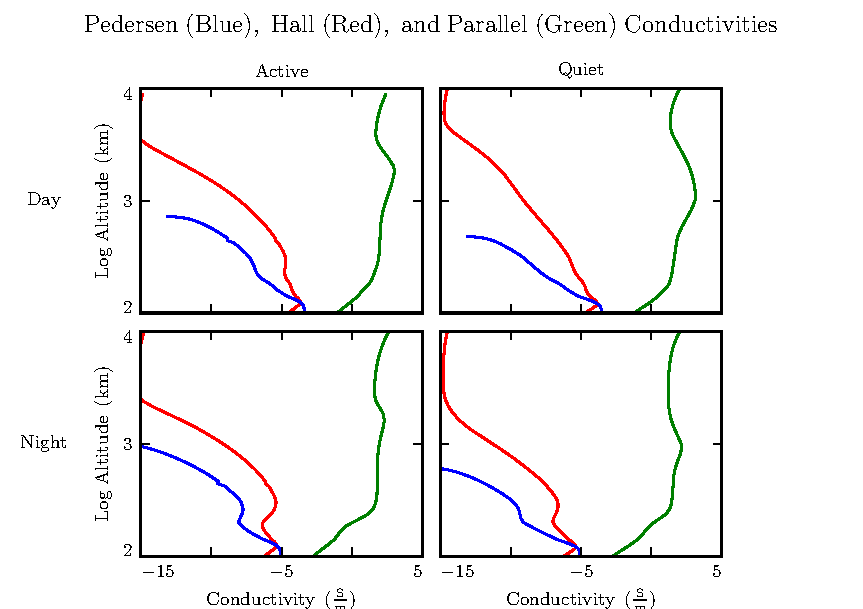
\includegraphics[width=\textwidth]{figures/sigma.pdf}
    \caption[Ionospheric Conductivity Profiles]{
      Ionospheric conductivity profiles, adapted by Lysak\cite{lysak_2013} from Appendix B of Kelley's textbook\cite{kelley_1989}. 
    }
    \label{fig_sigma}
\end{figure}

\todo{What is the height-interated conductivity for each profile? }

% -----------------------------------------------------------------------------
% -----------------------------------------------------------------------------
% -----------------------------------------------------------------------------
\subsection{\Alfven Speed}

The \Alfven speed is computed from Kelley's low-density profile, modified to take into account the local density. The density, in turn, is the sum of a plasmaspheric profile and a high-latitude auroral profile. 
\begin{align}
  \ep &= \text{(low-density tabulated value)} + \frac{ n \bar{m} }{B_0^2}
\end{align}

\todo{What's a clean way of showing the low-density \ep that we read in? }

\todo{Above the profile, Bob scales the value that's read in as $r^5$ or something. Is there a citation for that? }

Where $\bar{m}$ is the ambient mean molecular mass and $B_0$ is the zeroth-order magnetic field strength, $B_0 = \SI{3.11e4}{\nano\tesla} \lr{ \frac{R_E}{r} }^3 \sqrt{ 1 + 3 \cos^2 \theta }$. Note that \SI{3.11e4}{\nano\tesla} is the value of the Earth's magnetic field at the equator on Earth's surface. 

\todo{Cite this number? }

Note that we do not scale the electric constant to units of $\ez$. 

The \Alfven speed is then computed per \cref{def_basics}, $\va^2 \equiv \frac{1}{\mz \ep}$. 

\todo{Put up a plot of the four \Alfven speed profiles. Show the dipole, or zoom in on the ionosphere? }

\todo{Shouldn't the \Alfven speed profiles be brought up early on, since they're necessary for discussions about evanescence at large \azm in \cref{ch_math}? }

\todo{Explain in this section how we figure out the time step. }

% =============================================================================
% =============================================================================
% =============================================================================
\section{Maxwell's Equations}
  \label{sec_eqns}

The model simulates the evolution of electric and magnetic fields in accordance with Maxwell's equations. Specifically, magnetic fields are advanced using \farlaw, and electric fields with \amplaw. Kirchhoff's formulation of \ohmlaw ($\vec{J} = \tensor{\sigma} \cdot \vec{E}$) is used to eliminate the explicit current dependence in \amplaw. 
\begin{align}
  \label{def_eqns}
  \ddt \vec{B} &= - \curl{E} &
  \tensor{\epsilon} \cdot \ddt \vec{E} &= \frac{1}{\mu_0} \curl{B} - \tensor{\sigma} \cdot \vec{E}
\end{align}

% -----------------------------------------------------------------------------
% -----------------------------------------------------------------------------
% -----------------------------------------------------------------------------
\subsection{Notation and Optimization}

Algebra is carried out on paper, producing expressions where each field value is a linear combination of previous field values. These coefficients are computed before the main loop begins. This offers a significant reduction in floating point operations each iteration. 

The \assign operator is used to indicate assignment, rather than equality. Values on the left are new, and those on the right are old. New and old magnetic field values are offset by \dt; electric field values staggered by $\frac{\dt}{2}$. As an example of this notation, \cref{def_assign} integrates \farlaw over a time step, assuming that the curl of the electric field varies slowly compared to \dt: 
\begin{align}
  \label{def_assign}
  \begin{split}
  \int_0^{\dt} dt \, \ddt \vec{B} &= - \displaystyle\int_0^{\dt} dt \, \curl{E} \\ 
  \left. \vec{B} \right|_{\dt} - \left. \vec{B} \right|_0 &= \left. - \dt \, \curl{E} \right|_{ \frac{\dt}{2} } \\
  \vec{B} &\assign \vec{B} - \dt \, \curl{E}
  \end{split}
\end{align}

It's also beneficial to store the curl of each field, rather than take derivatives on the fly. The following sections make use of the shorthand $\vec{C} \equiv \curl{E}$ and $\vec{F} \equiv \curl{B}$. Or, recalling \cref{jacobian_usage}, 
\begin{align}
  \label{def_curls}
  C^i & = \frac{ \varepsilon^{ijk} }{\jac} \dd{\lysakj} E_k &
  F^i & = \frac{ \varepsilon^{ijk} }{\jac} \dd{\lysakj} B_k
\end{align}

Only covariant field components are stored. Only contravariant curl components are stored. This cuts down on memory use, while also eliminating the time spent rotating between bases; those operations are built into the precomputed coefficients. 

% -----------------------------------------------------------------------------
% -----------------------------------------------------------------------------
% -----------------------------------------------------------------------------
\subsection{Magnetic Fields}

Taking advantage of the shorthand defined in \cref{def_curls}, \farlaw is simply written
\begin{align}
  \label{farlaw_ijk}
  \ddt B^i &= - C^i
\end{align}

Or, using the metric tensor to cast the magnetic field in terms of its covariant components, and writing out each coefficient explicitly,
\begin{align}
  \begin{split}
  B_1 &\assign B_1 - g_{11} \, \dt \, C^1 - g_{13} \, \dt \, C^3 \\
  B_2 &\assign B_2 - g_{22} \, \dt \, C^2 \\
  B_3 &\assign B_3 - g_{31} \, \dt \, C^1 - g_{33} \, \dt \, C^3
  \end{split}
\end{align}


% -----------------------------------------------------------------------------
% -----------------------------------------------------------------------------
% -----------------------------------------------------------------------------
\subsection{Electric Fields}
  \label{sec_e}

\amplaw, can be solved with integrating factors. From \cref{def_eqns}, 
\begin{align}
  \tensor{\epsilon} \cdot \ddt \vec{E} &= \frac{1}{\mu_0} \curl{B} - \tensor{\sigma} \cdot \vec{E}
\end{align}

The permittivity tensor is diagonal, and so can be trivially inverted. 
\begin{align}
  \label{amp_tensor}
  \lr{ \tensor{\Omega} + \tensor{ \mathbb{I} } \ddt } \cdot \vec{E} &= \tensor{v}^2 \cdot \vec{F}
\end{align}

Where $\tensor{ \mathbb{I} }$ is the identity tensor and in \x-\y-\z coordinates, 
\begin{align}
  \tensor{v}^2 &\equiv \frac{1}{\mz} \tensor{\epsilon}^{-1} = 
    \mmm{\va^2}{0}{0}
        {0}{\va^2}{0}
        {0}{0}{c^2}
  && \text{and} &
  \tensor{\Omega} &\equiv \tensor{\epsilon}^{-1} \cdot \tensor{\sigma} = 
    \mmm{ \frac{\sp}{\ep} }{ -\frac{\sh}{\ep} }{0}
        { \frac{\sh}{\ep} }{ \frac{\sp}{\ep} }{0}
        {0}{0}{ \frac{\sz}{\ez} } 
\end{align}

Using integrating factors, \cref{amp_tensor} gives
\begin{align}
  \vec{E} &\assign \exp \arg{ -\tensor{\Omega} \; \dt } \cdot \vec{E} + \dt \, \tensor{v}^2 \cdot \exp \arg{ -\tensor{\Omega} \; \tfrac{\dt}{2} } \cdot \vec{F}
\end{align}

\todo{Do we need to be careful here about the difference between a matrix and a tensor? }

The tensor exponential can be evaluated by considering the diagonal and off-diagonal terms separately. 
\begin{align}
  \tensor{\Omega} &= \tensor{\Omega}'
    + \frac{\sh}{\ep} 
    \mmm{0}{-1}{0}
        {1}{0}{0}
        {0}{0}{0} && \text{where} &
  \tensor{\Omega}' &=
    \mmm{ \frac{\sp}{\ep} }{0}{0}
        {0}{ \frac{\sp}{\ep} }{0}
        {0}{0}{ \frac{\sz}{\ez} }
\end{align}

Note that tensors are remarkably well-behaved when exponentiated\cite{hall_2015}, particularly since $\tensor{\Omega}'$ is diagonal, and thus they commute. 
\begin{align}
  \exp \arg{ \tensor{T} } &= \displaystyle\sum_n \frac{1}{ n! } \tensor{T}^n && \text{and} & \exp \arg{ \tensor{T} + \tensor{T}' } &= \exp \arg{ \tensor{T} } \exp \arg{ \tensor{T}' }
\end{align}

The off-diagonal terms collapse into sines and cosines, indicating a rotation about \z. 
\begin{align}
  \label{amp_final}
  \vec{E} &\assign \exp \arg{ -\tensor{\Omega}' \; \dt } \cdot \tensor{R}_z \arg{ \tfrac{-\sh \dt}{\ep} } \cdot \vec{E}
   + \dt \, \tensor{v}^2 \cdot \exp \arg{ -\tensor{\Omega}' \; \tfrac{\dt}{2} } \cdot \tensor{R}_z \arg{ \tfrac{-\sh \dt}{2 \ep} } \cdot \vec{F}
\end{align}

Where 
\begin{align}
  \tensor{R}_z \arg{\theta} &= 
  \mmm{\cos\theta}{-\sin\theta}{0}
      {\sin\theta}{\cos\theta}{0}
      {0}{0}{1}
\end{align}

The parallel term of term of \cref{amp_final} is simply
\begin{align}
  E_\parallel \assign E_\parallel \exp \arg{ \tfrac{- \sz \dt}{\ez} } + c^2 \dt F_\parallel \exp \arg{ \tfrac{- \sz \dt}{2 \ez} }
\end{align}

Or, in covariant terms, 
\begin{align}
  \label{amp_para}
  E_3 \assign E_3 \exp \arg{ \tfrac{- \sz \dt}{\ez} } + c^2 \dt \lr{ g_{31} F^1 + g_{33} F^3 } \exp \arg{ \tfrac{- \sz \dt}{2 \ez} }
\end{align}

For the ionospheric profiles and time steps employed by this model, $\frac{\sz \dt}{\ez}$ is never smaller than $10^3$. As a result, $\exp \arg{ \frac{- \sz \dt}{\ez} }$ is far too small to be stored in a double precision variable. That is, this simulation takes $E_\parallel$ (and, equally, $E_3$) to be uniformly zero. 

This, obviously, precludes any discussion of parallel electric fields or parallel currents. These topics are revisited in \cref{ch_inertia}. 

Not unrelatedly, recalling the definition of the plasma frequency and parallel conductivity from \cref{def_basics}, $\frac{\sz}{\ez}$ can also be written $\frac{\op^2}{\nu}$. 

The plasma frequency is very fast. 

The perpendicular components of \cref{amp_final}, mapped from the physical basis to the contravariant basis (per \cref{def_xyz_directions}) to the covariant basis (per \cref{metric_usage}), give
\begin{alignat}{6}
  \label{e1_final}
  & E_1 + \frac{ g^{13} }{ g^{11} } && E_3 \assign &&   && E_1 && \cos \arg{ \tfrac{- \sh \dt}{\ep} } \exp \arg{ \tfrac{- \sp \dt}{\ep} } &&  \notag \\
  &                                 &&             && + && E_2 && \sin \arg{ \tfrac{- \sh \dt}{\ep} } \exp \arg{ \tfrac{- \sp \dt}{\ep} } &&  \sqrt{ \frac{ g^{22} }{ g^{11} } } \notag \\
  &                                 &&             && + && E_3 && \cos \arg{ \tfrac{- \sh \dt}{\ep} } \exp \arg{ \tfrac{- \sp \dt}{\ep} } &&  \frac{ g^{13} }{ g^{11} } \\
  &                                 &&             && + && F^1 && \cos \arg{ \tfrac{- \sh \dt}{2\ep} } \exp \arg{ \tfrac{- \sp \dt}{2\ep} } &&  \frac{\va^2 \dt}{ g^{11} } \notag \\
  &                                 &&             && + && F^2 && \sin \arg{ \tfrac{- \sh \dt}{2\ep} } \exp \arg{ \tfrac{- \sp \dt}{2\ep} } &&  \frac{\va^2 \dt}{ \sqrt{ g^{11} g^{22} } } \notag \\
  \intertext{and}
  \label{e2_final}
  & && E_2 \assign && - && E_1 && \sin \arg{ \tfrac{- \sh \dt}{\ep} } \exp \arg{ \tfrac{- \sp \dt}{\ep} } &&  \sqrt{ \frac{ g^{11} }{ g^{22} } } \notag \\
  & &&             && + && E_2 && \cos \arg{ \tfrac{- \sh \dt}{\ep} } \exp \arg{ \tfrac{- \sp \dt}{\ep} } &&  \notag \\
  & &&             && - && E_3 && \sin \arg{ \tfrac{- \sh \dt}{\ep} } \exp \arg{ \tfrac{- \sp \dt}{\ep} } &&  \frac{ g^{13} }{ \sqrt{ g^{11} g^{22} } } \\
  & &&             && - && F^1 && \sin \arg{ \tfrac{- \sh \dt}{2\ep} } \exp \arg{ \tfrac{- \sp \dt}{2\ep} } &&  \frac{\va^2 \dt}{ \sqrt{ g^{11} g^{22} } } \notag \\
  & &&             && + && F^2 && \cos \arg{ \tfrac{- \sh \dt}{2\ep} } \exp \arg{ \tfrac{- \sp \dt}{2\ep} } &&  \frac{\va^2 \dt}{ g^{22} } \notag
\end{alignat}

The $E_3$ terms can be ignored at present, but \cref{ch_inertia} references back to them. 

% =============================================================================
% =============================================================================
% =============================================================================
\section{Driving}
  \label{sec_driving}

If no energy is added, the simulation is pretty boring. Everything just stays zero. 

% -----------------------------------------------------------------------------
% -----------------------------------------------------------------------------
% -----------------------------------------------------------------------------
\subsection{Outer Boundary Compression}

Driving from the outer boundary is the traditional way to do it. 

\todo{Cite and briefly explain past work done with compressional driving. This is what most of Bob's papers are, right? }

As discussed in \cref{sec_math_implications}, \Alfven waves become guided when the azimuthal modenumber is large. The energy all stays close to the outer boundary. No field line resonances of significant strength are created within the magnetosphere. 

\todo{Show a plot of compressional driving, maybe day and night, as \azm increases. Mean energy density over time? Something that shows the recession of waves away from the middle of the simulation. }

Compressional driving is applied by setting the value of $B_3$ at the outer boundary. 

A compression might reasonably be expected to drive waves with long azimuthal wavelengths. However, there is some indication that waves with short azimuthal wavelength can be driven as well, such as through Kelvin-Helmholtz interactions. 

\todo{Find this claim again and cite it. }

% -----------------------------------------------------------------------------
% -----------------------------------------------------------------------------
% -----------------------------------------------------------------------------
\subsection{Ring Current Modulation}

Pc4 pulsations with high azimuthal modenumber are known to be driven from within the magnetosphere, such as through drift-resonant interactions with energetic radiation belt and ring current particles. 

\todo{Cite. }

Substorm injection can cause localized ring current behavior. 

\todo{UNH was looking at this at AGU. Check if they have published yet. }

During geomagnetically active times, the ring current is a dynamic region. It's easy to imagine localized perturbations. 

It's difficult to estimate how large such perturbations might be. The following is a kludgey estimate. 

\todo{Plot of Sym-H and its Fourier modes. 1 June 2013. 17 March 2015. 22 June 2015. 17 March 2013. Fit at the ``top'' of the $\frac{1}{f}$ noise. (``Pink noise''?) }

Sym-H is like Dst, but with greater time resolution. 

The noise suggests that a Fourier component with a period of about \SI{1}{\minute} could have an amplitude around \SI{e-3}{\nano\tesla}. 

If the driving is delivered at $L=5$, with a standard deviation of \SI{0.5}{\RE} in the radial direction and \SI{5}{\degree} angularly, that corresponds to a current density of about \SI{4e-4}{\uA/\meter\squared}. This comes from approximating the ring current as a ring of current. Of course, Sym-H is measured at Earth's surface, not at the center of the ring; this gives a geometric factor of about two. 

\todo{What electric field magnitude does this correspond to? }

Current driving is applied by adding an additional current term. \amplaw becomes
\begin{align}
  \tensor{\epsilon} \cdot \ddt \vec{E} &= \frac{1}{\mu_0} \curl{B} - \tensor{\sigma} \cdot \vec{E} - \vec{J}_{drive}
\end{align}

And this driving term is absorbed into the curl by revising \cref{def_curls} from $\vec{F} \equiv \curl{B}$ to $\vec{F} \equiv \curl{B} - \vec{J}_{drive}$. (As a result, \cref{e1_final,e2_final} do not change.)

Notably, Sym-H is a global quantity; it's not ideally suited for making estimates of localized inhomogeneity. 

Furthermore, Sym-H has a time resolution of \SI{1}{\minute}. It can hardly be said to carry information about oscillations at frequencies of less than two minutes. 

Sym-H gives no way to estimate azimuthal modenumber. That's based on Pc4 observations. Dai\cite{dai_2015} observed modenumbers approaching \num{100}. 

A kludgey estimate is better than no estimate. 

% =============================================================================
% =============================================================================
% =============================================================================
\section{Boundary Conditions}
  \label{sec_bcs}

The grid can't go on forever. There have to be special cases at the edges. 


% -----------------------------------------------------------------------------
% -----------------------------------------------------------------------------
% -----------------------------------------------------------------------------
\subsection{Parity and Interpolation}

Computation takes place on a staggered grid. 

Field values are offset to ensure that most differences are centered. For example, $\ddt B_2$ depends on $\dd{\lysakx} E_3$ and $\dd{\lysakz} E_1$. If $B_2$ is defined at even $i$, $E_3$ is defined at odd $i$, so that $B_2$ is defined on the same grid points as $\frac{ E_3 \lrb{i+1} - E_3 \lrb{i-1} }{ \lysakx \lrb{i+1} - \lysakx \lrb{i-1} }$. 

\todo{Make sure the example uses the currect parities. }

\todo{Find a citation for the wigglies that occur if field values are defined on all grid points, due to the weak coupling. This problem is apparently well-known. }

Values are sometimes needed off-parity. $E_1$ and $E_2$ are not defined at the same grid locations, but they are coupled directly by the Hall conductivity. And $B_1$ and $B_3$ are coupled by the non-orthogonality of the grid. When off-parity values are needed, they are interpolated from their neighbors. 

Differentiation and interpolation are good to second order on the nonuniform grid. Like the coefficients for Maxwell's equations, differentiation and interpolation weights are computed during setup to save time during iteration. 

Electric fields go to zero at the innermost and outermost field lines (Dirichlet boundary conditions). Magnetic fields have zero derivative (Neumann boundary conditions). For components not defined at the exact boundary, these rules are applied when differentiating or interpolating; they set the effective value just outside the grid. 

These boundary conditions can in principle cause nonphysical reflection at the boundary. In practice, that is not an issue. Wave activity is concentrated well away from the boundaries. In fact, reversing the Dirichlet and Neumann boundary conditions has little effect. 

(Of course, an inconsistent boundary condition -- like using the same boundary condition for a field and its derivative -- causes instability.)

% -----------------------------------------------------------------------------
% -----------------------------------------------------------------------------
% -----------------------------------------------------------------------------
\subsection{Coupling to the Atmosphere}

Conditions at the ionospheric boundaries are set by coupling to the atmosphere. This also allows the computation of ground fields. 

It's reasonable to approximate the atmosphere as a perfect insulator, giving $\curl{B}=0$. Combining with $\div{B}=0$ per Maxwell's equations, ensures the existence of a scalar magnetic potential $\Psi$ such that $\vec{B}=\grad{\Psi}$ and $\Psi$ satisfies Laplace's equation, $\nabla^2 \Psi = 0$. 

Laplace's equation can be solved analytically; in spherical coordinates, the solutions are spherical harmonics. However, a numerical solution is preferrable to ensure orthonormality on a discrete (and incomplete -- there are no grid points at the poles or equator) grid. After separating out the radial and azimuthal dependence in the usual way, the latitudinal component of Laplace's equation (in terms of $s \equiv - \sin^2 \theta$) is
\begin{align}
  \label{laplace}
  \lr{ 4 s^2 + 4s } \frac{d^2}{ds^2} Y_\ell + \lr{ 4 + 6 s } \frac{d}{ds} Y_\ell - \frac{\azm^2}{s} Y_\ell &= \ell \lr{ \ell + 1 } Y_\ell
\end{align}

Using centered differences to express the derivatives, \cref{laplace} is a system of linear equations, one per field line. It can be solved numerically for eigenvalues $\ell \lr{\ell + 1}$ and eigenvectors (harmonics) $Y_\ell$. In terms of those harmonics, and noting that the model uses a fixed azimuthal modenumber \azm, $\Psi$ between $R_E$ and $R_I$ can be expressed
\begin{align}
  \label{psi_expansion}
  \Psi \arg{r, \theta, \phi} &= \displaystyle\sum_\ell \lr{ \alpha_\ell \, r^\ell + \beta_\ell \, r^{-\ell - 1} } Y_\ell \arg{\theta} \exp \arg{i \azm \phi}
\end{align}

As a boundary condition for $\Psi$, Earth's crust is assumed to be a perfect conductor, forcing the magnetic field at the boundary to be perfectly horizontal. That is, $B_r = \dd{r} \Psi = 0$. Then, noting that the harmonics $Y_\ell$ are orthonormal (so each term of the sum must be zero), 
\begin{align}
  \label{beta_solution}
  \beta_\ell &= \frac{\ell}{\ell + 1} R_E^{2 \ell + 1} \alpha_\ell
\end{align}

Note that the explicit $\phi$ dependence has been dropped. The entire simulation shares a fixed modenumber, so it's sufficient to find $\Psi$ at $\phi=0$. 

At the top of the atmosphere, the radial magnetic field is again used as a boundary condition, this time to compute the weights $\alpha_\ell$. 

\todo{Something something thin horizontal current sheet at $R_I$. }

Taking the shorthand $\lambda_I \equiv \frac{R_E}{R_I} \sim \num{0.975}$
\begin{align}
  B_r &= \displaystyle\sum_\ell \ell \, \alpha_\ell \, R_I^{\ell-1} \, \lr{ 1 - \lambda_I^{2 \ell - 1} } Y_\ell
\end{align}

\todo{Settle on good notation for taking the inner product of harmonics. It's a vector in the sense that it's a one-dimensional array of values, but not in the physical sense. Indexing -- $B_r\lrb{i}$ -- also seems awkward. }

The sum can be collapsed by ``integrating" over a harmonic. The inverse harmonics are obtained by inverting the eigenvector matrix. Then $Y_\ell \cdot Y_{\ell'}^{-1} = \delta_{\ell \ell'}$ by construction. 
\begin{align}
  \label{alpha_solution}
  \alpha_\ell &= \frac{ 1 }{\ell \, R_I^{\ell-1} } \frac{ B_r \cdot Y_\ell^{-1} }{ 1 + \lambda_I^{2 \ell + 1} }
\end{align}

Combining \cref{psi_expansion,beta_solution,alpha_solution} allows the expression of $\Psi$ at the top and bottom of the atmosphere as a linear function of the radial magnetic field at the boundary. 
\begin{align}
  \label{psi_final}
  \begin{split}
  \Psi_E &= \displaystyle\sum_\ell Y_\ell \; \frac{R_I}{\ell} \frac{ \frac{2 \ell - 1}{\ell - 1} \lambda^\ell }{ 1 - \lambda_I^{2 \ell + 1} } B_r \cdot Y_\ell^{-1} \\
  \Psi_I &= \displaystyle\sum_\ell Y_\ell \; \frac{R_I}{\ell} \frac{ 1 + \frac{\ell}{\ell - 1} \lambda_I^{2 \ell + 1} }{ 1 - \lambda_I^{2 \ell + 1} } B_r \cdot Y_\ell^{-1}
  \end{split}
\end{align}

Magnetic fields are evaluated from $\Psi$ per 
\begin{align}
  B_1 &= \dd{\lysakx} \Psi &
  B_2 &= \dd{\lysaky} \Psi
\end{align}

Note that $B_1$ and $B_2$ are horizontal; per \cref{def_rqf_directions}, they are proportional to $B_\theta$ and $B_\phi$ respectively. 

At the ground, field values are purely output. 

Horizontal magnetic field values at the top of the ionosphere, on the other hand, are used as boundary conditions. Assuming there is no vertical component to the ionospheric current sheet, the electric field values at the ionospheric edge of the grid are dictated by the jump in horizontal magnetic field between the bottom of the grid and the top of the atmosphere. 
\begin{align}
  \mz \, \tensor{\Sigma} \cdot \vec{E} &= \left. \displaystyle\lim_{\dr \rightarrow 0} \, \hat{r} \! \times \! \vec{B} \, \right|^{R_I + \dr}_{R_I - \dr}
\end{align}

\todo{Bob's citations for the ionospheric jump conditions: Fujita and Tamao 1988, Yosikawa and Itonaga 1996, 2000, Lysak and Song 2001, Sciffer and Waters 2002. It basically comes from integrating \amplaw, so half a dozen citations seems like overkill. }







\chapter{Numerical Results}
  \label{ch_results}

\todo{This chapter is the real moneymaker. The overarching motivation for this work is that Pc4 pulsations vary in interesting ways with respect to azimuthal modenumber, and that prior models have been unable to give a good picture of that behavior. }

%\todo{Do we every check E/B against $\Sigma_P / \mz$? }

%\todo{Do we see a difference between \vec{k} (momentum) and the group velocity? Poynting flux will always be pretty much along the field line, since $B_3$ is small and $E_3$ is zero, but the wave vector need not be. This is a question of coupling/converting to compressional waves, I guess. }

%\todo{Look at McKenzie and Westphal. Waves incident on the bow shock, etc, at weird angles. }

%\todo{Look at the E to B ratio. Compare to the \Alfven speed and to the height-integrated Pedersen conductivity. }

% -----------------------------------------------------------------------------
% -----------------------------------------------------------------------------
% -----------------------------------------------------------------------------
\section{Finite Poloidal Lifetimes}
  \label{sec_lifetimes}

In his 1974 paper, Radoski argues that a poloidally-polarized wave should asymptotically rotate to the toroidal polarization\cite{radoski_1974} as a result of the curved derivative in the meridional plane. The question of finite poloidal lifetimes is considered further in a 1995 paper by Mann and Wright\cite{mann_1995}. Their numerical work used a straightened field line, with an \Alfven speed gradient in the ``radial'' direction. They also found a rotation over time from poloidal to toroidal polarization, with the characteristic time proportional to the azimuthal modenumber. 

\todo{Ding et al\cite{ding_1995} did similar work just before Mann and Wright, but results were less clear, possibly due to issues with grid resolution (as discussed in \cite{mann_1995}). }

\todo{Mann and Wright looked specifically at second harmonics. This work is on first harmonics. (In principle Tuna allows arbitrary driving waveforms and spatial distributions.) }

The present section builds on the aforementioned results by relaxing several of their nonphysical assumptions. First, Tuna's geometry (as described in \cref{ch_model}) is far more realistic than Radoski's half-cylinder or the box model used by Mann and Wright. Magnetic field lines are dipolar. \Alfven speed is based on an empirical profile, and varies along and across field lines. Next, the present results feature driving delivered over time through perturbation of the ring current; past work has instead considered the evolution of an initial condition. Finally, the present model includes a height-resolved ionosphere (rather than perfectly-reflecting boundaries). The ionospheric conductivity provides a direct coupling between the poloidal and toroidal modes, in addition to dissipating energy. 

Each subplot in \cref{fig_U_day,fig_U_day_big,fig_U_night} is analogous to Mann's Figure 3. Blue lines show the total energy in the poloidal mode as a function of time. Red lines show toroidal energy. Runs are organized such that driving frequency is constant down each column, and azimuthal modenumer is constant across each row. Axis bounds are held constant across all subplots. 

Energy is computed per Poynting's theorem, with due consideration of the unusual geometry. Energy density is integrated over the meridional plane, but not in the azimuthal direction, giving units of gigajoules per radian; more than anything else, this serves as a reminder that the waves under consideration are azimuthally localized. 
\begin{align}
  \label{def_energy}
  U_P &= \displaystyle\int \frac{d\lysakx d\lysakz}{2 \mz \jac} \lr{ B_x^2 + \frac{1}{\va^2} E_y^2} &
  U_T &= \displaystyle\int \frac{d\lysakx d\lysakz}{2 \mz \jac} \lr{ B_y^2 + \frac{1}{\va^2} E_x^2} 
\end{align}

The twenty-eight runs shown in \cref{fig_U_day} use a high-conductivity profile, corresponding to the dayside with high solar activity. 

\begin{figure}[!htb]
    \centering
    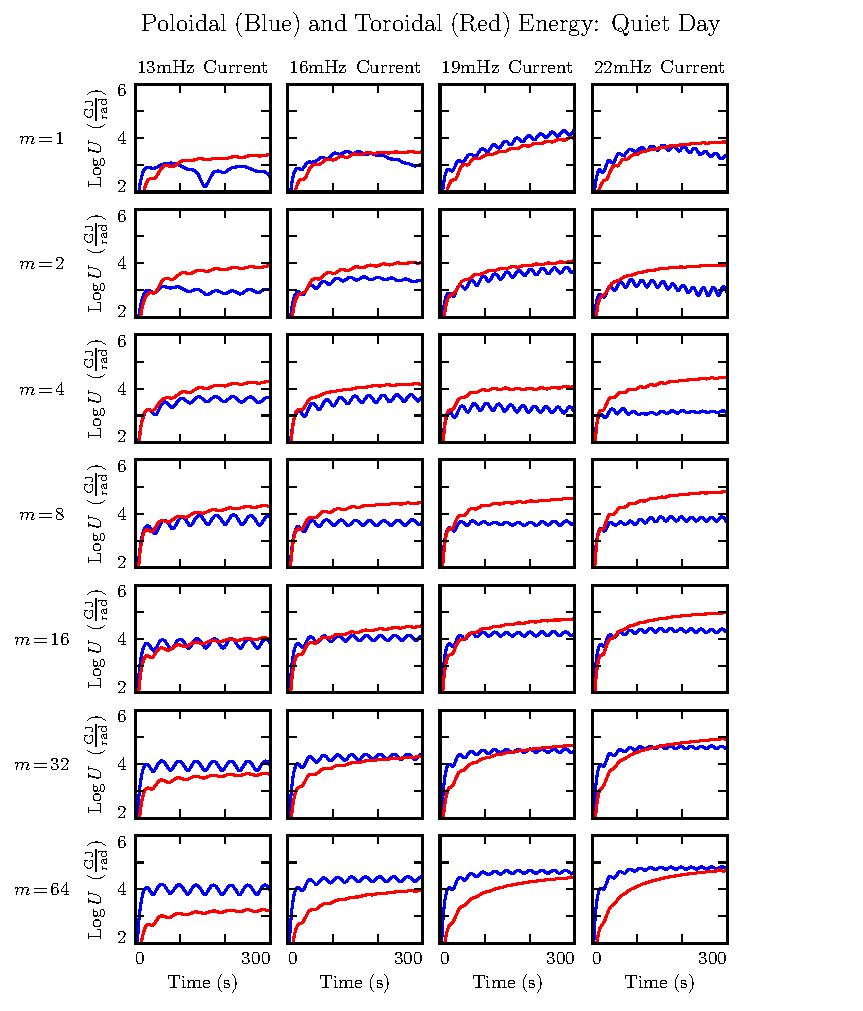
\includegraphics[width=\textwidth]{figures/U_day.pdf}
    \caption[Poloidal and Toroidal Energy: Quiet Day]{
      \todo{MAKE THIS PLOT WITH MODEL 2. }
    }
    \label{fig_U_day}
\end{figure}

The fact that \cref{fig_U_day} includes red (toroidal energy) curves at all speaks to the coupling of the poloidal and toroidal modes. As discussed in \cref{ch_model}, driving in Tuna is delivered purely into the poloidal electric field (as a proxy for the azimuthal current). 

As expected, the rotation from poloidal to toroidal is slowest at large azimuthal modenumbers. The toroidal energy overtakes the poloidal energy within a single drive period at $\azm=4$; with $\azm=64$, the most of the energy is in the poloidal mode for \about10 driving periods. However, the relationship between azimuthal modenumber and rotation timescale is not linear, as was suggested by Mann and Wright. Instead, the rotation is fastest at $\azm=4$. 

This hints at two competing effects. \todo{Probably the Hall conductivity? Get these runs in here. Note also that in \cref{ch_inertia} we talked about how the Hall conductivity isn't add a significant imaginary component to $B_x$, etc. }

\begin{figure}[!htb]
    \centering
    
\includegraphics[width=\textwidth]{figures/placeholder.jpg}
    \caption[Poloidal and Toroidal Energy: Quiet Day, No Hall Conductivity]{
      \todo{CARRY OUT THESE RUNS. } 
    }
    \label{fig_U_day_nosigh}
\end{figure}

The total energy in the system is asymptotically determined by the balance between the energy input (from driving) and the energy loss (through Joule dissipation in the ionosphere). When the driving frequency is not particularly close to the local \Alfven frequency, the energy reaches its asymptotic value quickly. When those frequencies align closely, energy accumulates over a larger number of drive periods, and the asymptotic value is larger. 

The system's resonant frequency (for a fundamental poloidal mode at $L=5$) is affected significantly by the size of the plasmasphere. In \cref{fig_U_day}, with the plasmapause at $L_{PP}=4$, the system resonates at \SI{19}{\mHz} at low \azm; as \azm becomes large, the resonant frequency is closer to \SI{22}{\mHz}. \cref{fig_U_day_big} shows the effect of moving the plasmapause to $L_{PP}=5$: resonance is closer to \SI{16}{\mHz}. The runs are otherwise identical to those shown in \cref{fig_U_day}. 

\begin{figure}[!htb]
    \centering
    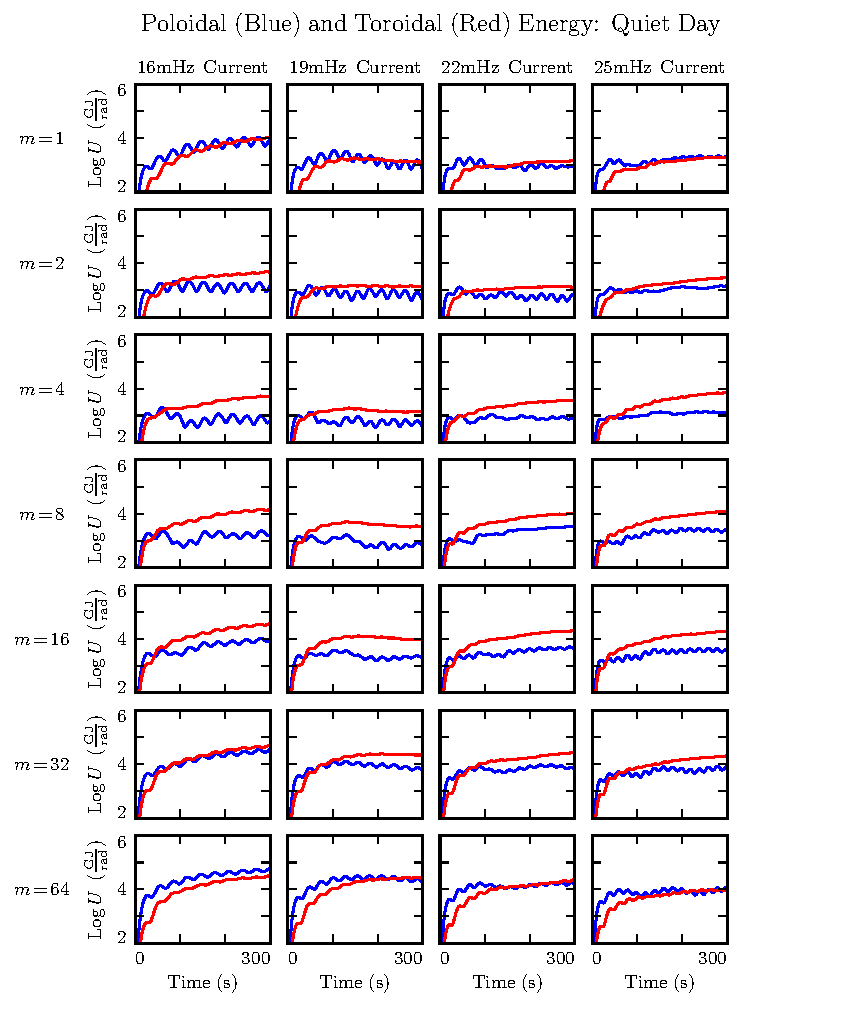
\includegraphics[width=\textwidth]{figures/U_2_LPP_5.pdf}
    \caption[Poloidal and Toroidal Energy: Quiet Day, Large Plasmasphere]{
      Changing the position of the plasmapause has a significant effect on the \Alfven bounce time. \todo{FIX PLOT TITLE. } 
    }
    \label{fig_U_day_big}
\end{figure}

On the nightside, the picture changes significantly. 







\todo{This result shows agreement with -- and significant refinement of -- Mann's findings. In the case of large-but-finite ionospheric conductivity, dipole geometry, and realistic \Alfven speed profile, energy does asymptotically rotate from the poloidal mode to the toroidal mode. The rotation rate is strongly affected by azimuthal modenumber and, in the case of large-but-finite \azm, has a characteristic timescale in the tens of periods. The present work furthermore demonstrates that the rotation rate is affected by driving frequency (did Mann talk about this at all, or just work in normalized time?) }

In \cref{fig_U_night}, runs are carried out using a low-conductivity profile: quiet nightside. 

\begin{figure}[!htb]
    \centering
    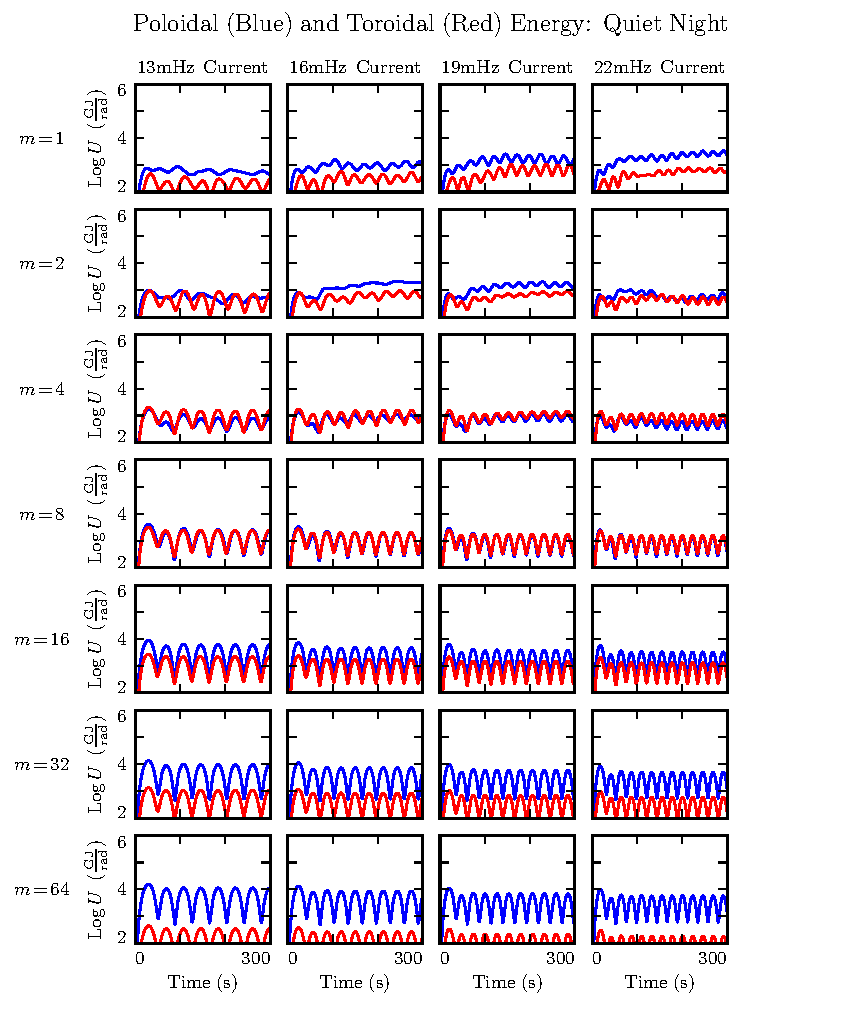
\includegraphics[width=\textwidth]{figures/U_4.pdf}
    \caption[Poloidal and Toroidal Energy: Quiet Night]{
      Driving is applied to the poloidal electric field. There is some rotation of energy to the toroidal mode (and less at high azimuthal modenumber), but the low ionospheric conductivity prevents energy from accumulating over time. 
    }
    \label{fig_U_night}
\end{figure}

\todo{Dissipation is much more important. It's fast enough to prevent an accumulation of energy over multiple wave periods. It looks like a damped-driven oscillator. }

\todo{Rotation from poloidal toroidal is still trying to happen. At high \azm, the asymptotic bounds for the toroidal energy are relatively low compared to the bounds of the poloidal energy. This indicates that dissipation is relatively fast compared to rotation. }

\todo{Previous considerations of poloidal lifetimes have been limited to the high conductivity regime. The present work demonstrates that the low conductivity regime exhibits qualitative differences. Ionospheric conductivity on the nightside is low enough that resonance does not develop, even in the case of ongoing driving. The dissipation timescale is comparable to the rotation timescale. Rather than aymoptotically accumulating energy in the toroidal mode, the oscillator asymptotically oscillates following the driving. This is relevant to the question of day-night asymmetry in the observation of field line resonances. }


% -----------------------------------------------------------------------------
% -----------------------------------------------------------------------------
% -----------------------------------------------------------------------------
\section{Spatial Distribution of Energy}
  \label{sec_shells}

Looking a bit deeper, it's possible to comment on the structure of the poloidal and toroidal modes, not just their magnitudes. The following commentary addresses the dayside; on the nightside, there's never much by the way of resonance. 

In \cref{fig_resonant_driving,fig_nonresonant_driving}, electromagnetic energy is binned by field line, averaged over volume (again, with respect to the Jacobian), and plotted as contours. All plots share a color scale. 

The poloidal mode and the toroidal mode exhibit qualitatively different behavior, related to the fact that energy rotates from poloidal to toroidal, and not back. 

At low \azm, energy rotates out of the poloidal mode so quickly that no resonance can form. 

At high \azm, the \Alfven wave is guided. If the driving frequency lines up with the resonant frequency where it's delivered, the poloidal mode resonates strongly. Otherwise, again, no energy accumulates. 

In no case does the poloidal mode demonstrate the ability to move energy across magnetic field lines. 

On the other hand, the toroidal mode does resonate, even if the driving isn't resonant (though in that case the response is of course stronger). The toroidal mode transports energy across field lines until it encounters resonance, then accumulates energy there. Often, resonances are seen in multiple locations due to the non-monotonic \Alfven bounce frequency as a function of $L$. 

% RESONANT DRIVING

\begin{figure}[H]
    \centering
    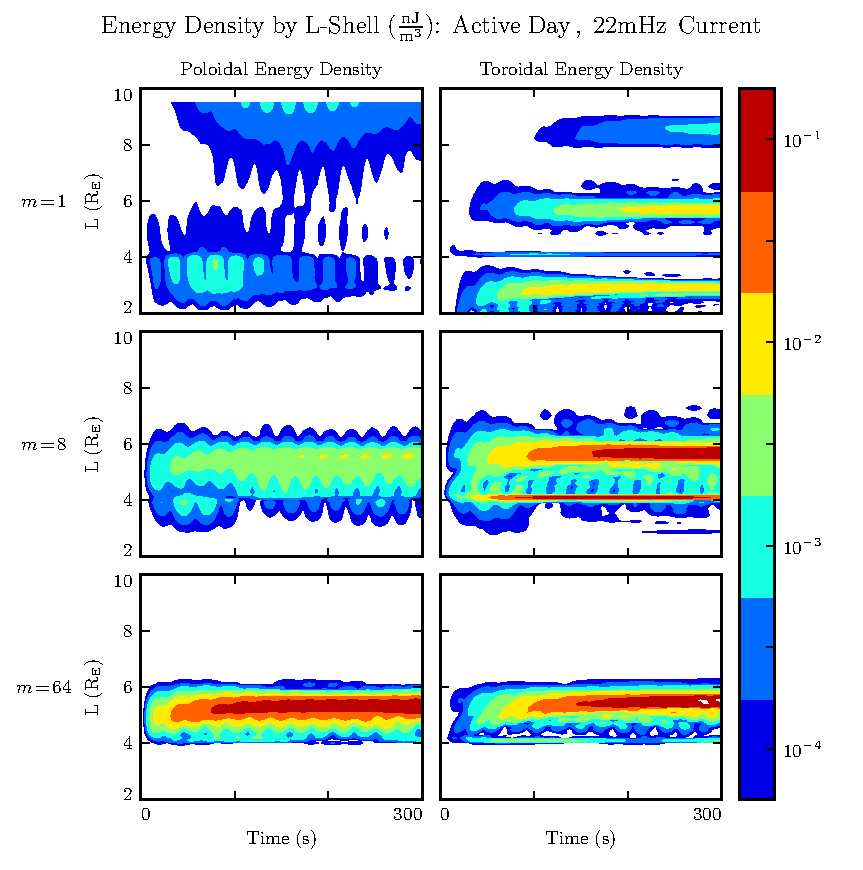
\includegraphics[width=\textwidth]{figures/layers_22mHz_1.pdf}
    \caption[Poloidal and Toroidal Energy Distribution: Resonant Driving]{
      If \azm is small, energy rotates to the toroidal mode too fast to form a poloidal resonance. If \azm is large, the \Alfven wave is guided, so it resonates only if the driving frequency lines up with the resonant frequency where it's applied. The result is just one big -- or perhaps even giant -- pulsation. If the driving lines up with a nearby field line, the toroidal mode goes crazy! Resonance inside the plasmasphere. Resonance at the plasmapause. Resonance at the driving location. And (weak) attempt at a higher harmonic further out. 
    }
    \label{fig_resonant_driving}
\end{figure}

\todo{Why is this exciting? }

\todo{Driving from inside the magnetosphere is novel. }

% NONRESONANT DRIVING




\begin{figure}[H]
    \centering
    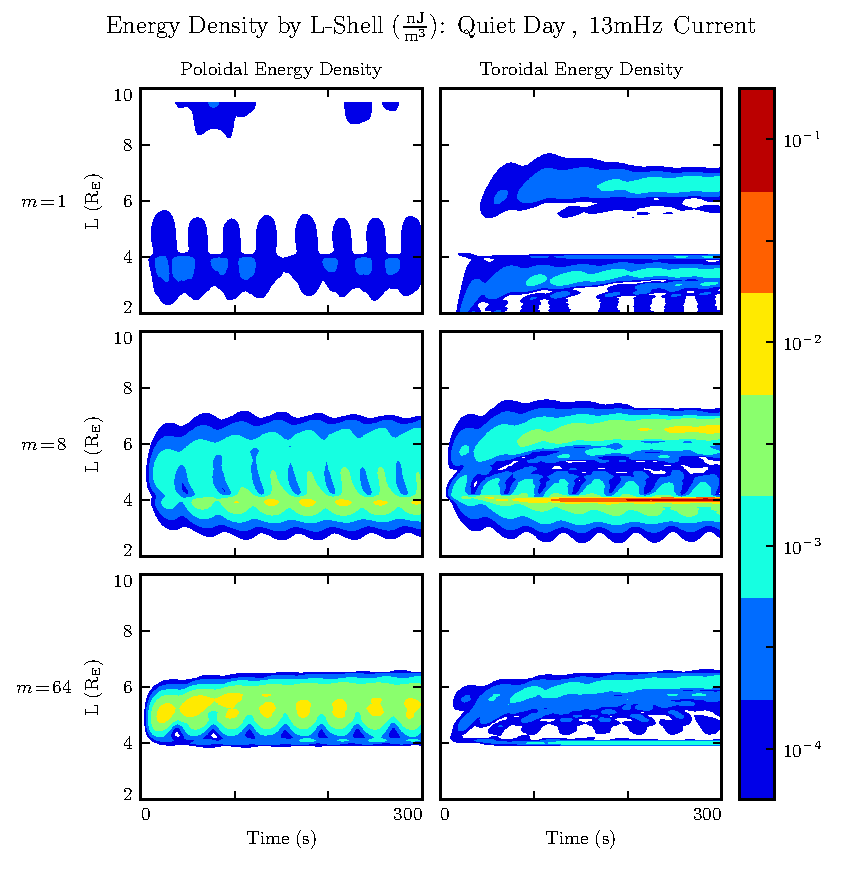
\includegraphics[width=\textwidth]{figures/layers_13mHz_2.pdf}
    \caption[Poloidal and Toroidal Energy Distribution: Nonresonant Driving]{
      When the driving frequency doesn't line up with the location where it's delivered, there's basically no response. There is no movement of energy to a resonant field line, so no energy can accumulate over the course of multiple rounds of driving. Even when not driven resonantly, the toroidal mode still makes the best of its situation. It steals what energy it can from the poloidal mode, carries it to the resonant $L$-shell, and gets to work. (In contrast, recall from \cref{fig_resonant_driving}, in this situation the poloidal mode just does not accumulate energy.)
    }
    \label{fig_nonresonant_driving}
\end{figure}

\todo{Why is this exciting? }









% =============================================================================
% =============================================================================
% =============================================================================
\section{Significance for Giant Pulsations}
  \label{sec_pgs}

Giant pulsations are (probably\cite{takahashi_2011}) fundamental mode poloidal Pc4 pulsations with frequencies around \SI{10}{\mHz} and azimuthal modenumbers around \num{20}. They are large, and can sometimes be observed on the ground. 

While this model makes no particular distinction between a giant pulsation and any other Pc4, the above results do line up with giant pulsation observations. 

Giant pulsations aren't seen at small \azm. As shown in \cref{sec_lifetimes}, low-\azm poloidal modes rotate to the toroidal mode too quickly to resonate effectively, even in the case of continuous driving at a locally-resonant frequency. The sweet spot seems to be around $\azm = 20$, more or less the same point where resonance becomes visible in \cref{fig_resonant_driving}. Admittedly, giant pulsations are typically closer to \SI{10}{\mHz} than \SI{22}{\mHz}. It seems likely that qualitatively similar results would be encountered if the driving were moved to an $L$-shell with a bounce time of \SI{10}{\mHz}. 


% GROUND SIGNATURES

\todo{\cite{takahashi_2011} talks significantly about the east-west polarization. }

Giant pulsations are seen at very large \azm, though not on the ground\cite{takahashi_2013}, due to damping by the ionosphere. 

Giant pulsations are most common on the dayside (particularly the morningside), during geomagnetically quiet times. Giant pulsation ground signatures are noted for their predisposition towards east-west polarization. 

In \cref{fig_ground_signatures}, the strongest east-west ground signatures is obtained on the geomagnetically quiet dayside, at \azm of 16 and 32. 

This seems to be a giant pulsation ``sweet spot'': the poloidal mode becomes stronger as \azm increases, but the ionospheric damping also increases. 

\begin{figure}[H]
    \centering
    \includegraphics[width=\textwidth]{figures/ground_16mHz.pdf}
    \caption[Dayside Ground Magnetic Fields]{
      The east-west component of magnetic ground signatures is peaked on the geomagnetically quiet dayside, at modenumbers around 16 to 32. This coincides nicely with observations of giant pulsations. Like the east-west component, the north-south ground signature is strongest on the quiet dayside; however, unlike the east-west component, the north-south component is weak when the modenumber is large. 
    }
    \label{fig_ground_signatures}
\end{figure}

Giant pulsations are monochromatic, and can be accompanied by ``multiharmonic toroidal waves''\cite{takahashi_2011}. Per \cref{sec_shells}, this is about what would be expected from a mishmash of poloidal driving. Poloidal modes of all frequencies rotate into the toroidal mode; resonant poloidal modes resonate; non-resonant poloidal modes become evanescent. 

Giant pulsations often drift azimuthally. This model can't resolve azimuthal drift directly, of course, but can fake it by looking at complex phase. There has been some indication (not shown) of complex phase rotation in ground magnetic fields. However, at the boundary, it's difficult to disentangle which values are imaginary to indicate an azimuthal offset, and which are imaginary because of Hall coupling. Investigation is ongoing. 









% =============================================================================
% =============================================================================
% =============================================================================
%\section{Electromagnetic Energy Gap}

%\todo{A preliminary search (and asking Bob) has not turned up anyone looking at this before, so it's hard to provide context. }

%Above, we considered the decay of energy from the poloidal mode to the toroidal mode. A natural follow up is, are there any other surprising trends in the distribution of energy?

%As it turns out, yes!

%In cases where the driving frequency does not line up with the local bounce frequency, energy doesn't accumulate particularly well in either the poloidal or the toroidal mode. Like a damped-driven oscillator, the system's behavior follows the input. 

%At low \azm, what energy there is divides itself more or less equally between the electric and magnetic fields. 

%As \azm increases, oddly, a gap appears. When the conductivity is high, the magnetic field holds more energy than the electric field. The disparity can be up to a factor of $\sim \num{3}$; that is, \SI{75}{\percent}. of the energy in the magnetic field, and \SI{25}{\percent} in the electric field. When conductivity is low, the opposite happens: energy concentrates in the electric field. 

%This lines up somewhat with what might be expected. When conductivity is low, it takes a larger electric field to induce the same current, and thus the same magnetic field. But it's not clear why this disparity only appears at large \azm, or why it does not appear when the driving is resonant. 

%Maybe it's a timing issue? A relationship between the bounce time (which is more or less indepedent of \azm) and the rotation time (which depends on \azm). 

%\todo{How is the compressional magnetic field brought into these calculations? It exists only at small \azm. It's never particularly large, it also gets added to the zeroth-order field before squaring. }

%\begin{figure}[H]
%    \centering
%    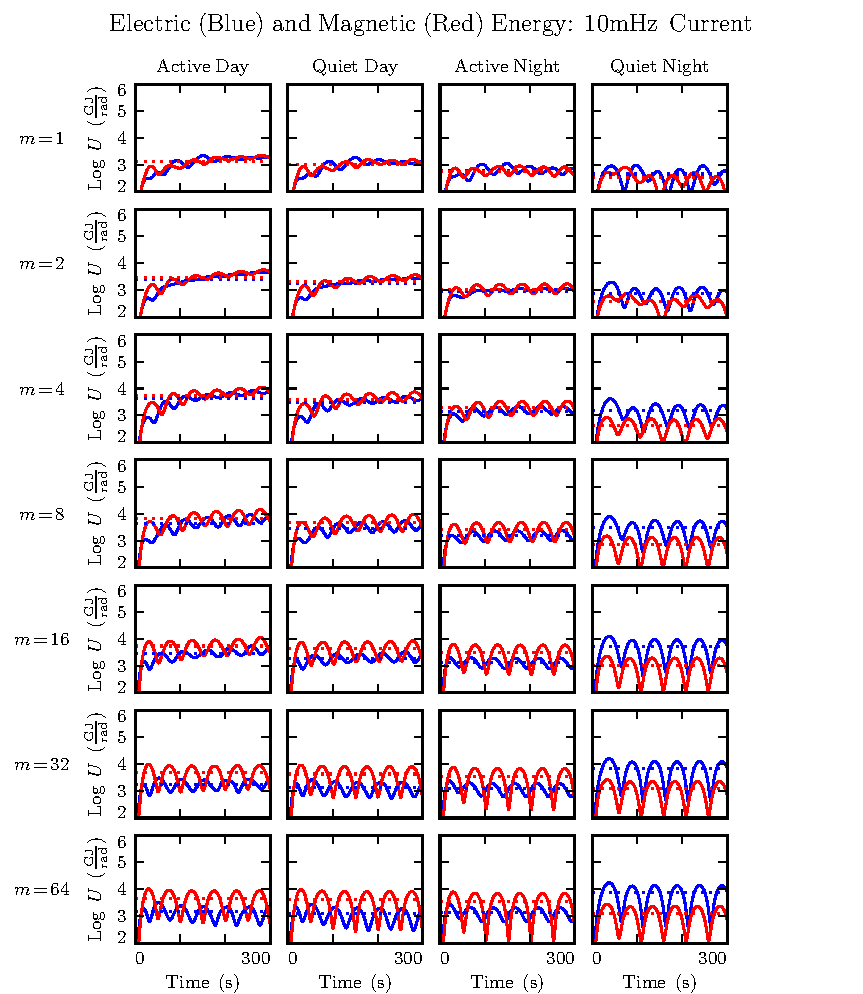
\includegraphics[width=\textwidth]{figures/U_BE_010mHz.pdf}
%    \caption[Current-Driven Electric and Magnetic Energy: 10mHz]{
%      In the absence of resonant driving, a disparity emerges at large \azm between the energy in the magnetic field and the energy in the electric field. The sign of the difference depends on the ionospheric conductivity. 
%    }
%    \label{fig_U_BE_010mHz}
%\end{figure}

%\begin{figure}[H]
%    \centering
%    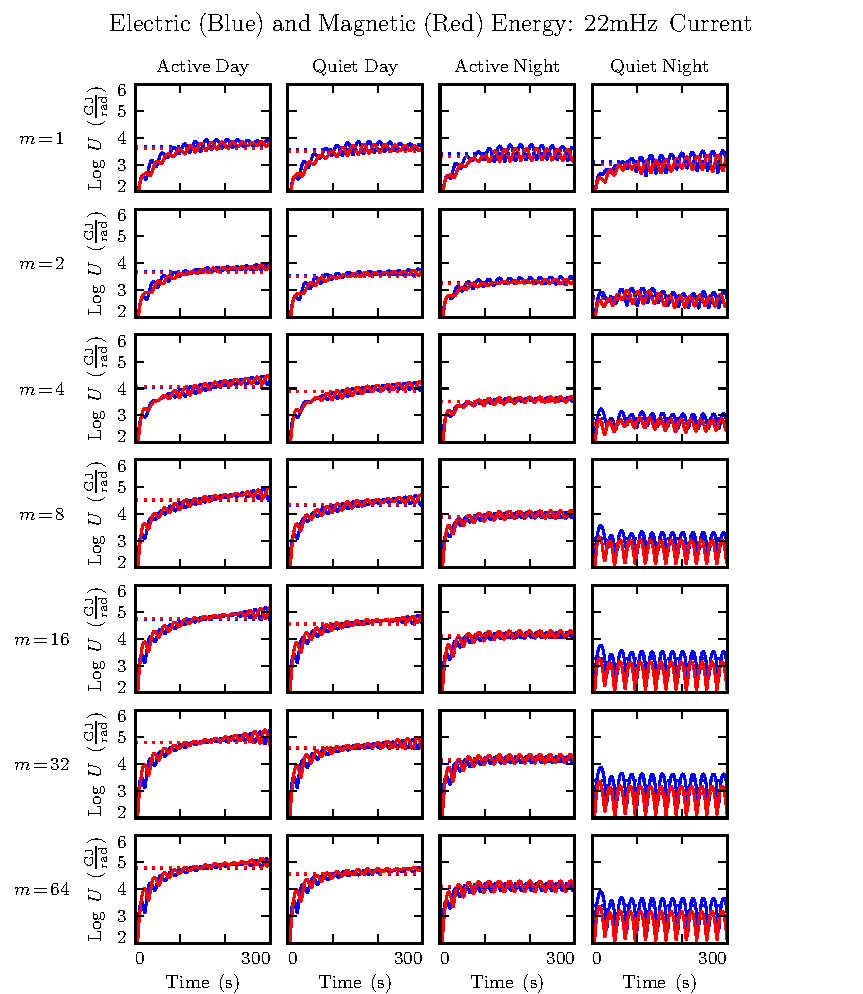
\includegraphics[width=\textwidth]{figures/U_BE_022mHz.pdf}
%    \caption[Current-Driven Electric and Magnetic Energy: 22mHz]{
%      When driving is resonant, energy is distributed almost exactly half-and-half between the electric and magnetic fields, regardless of \azm. The rightmost profile still shows a gap, likely because the ionospheric conductivity in that model is low enough that nothing ever resonates. 
%    }
%    \label{fig_U_BE_022mHz}
%\end{figure}














% %%%%%%%%%%%%%%%%%%%%%%%%%%%%%%%%%%%%%%%%%%%%%%%%%%%%%%%%%%%%%%%%%%%%%%%%%%%%%
% %%%%%%%%%%%%%%%%%%%%%%%%%%%%%%%%%%%%%%%%%%%%%%%%% Comparison of Model to Data
% %%%%%%%%%%%%%%%%%%%%%%%%%%%%%%%%%%%%%%%%%%%%%%%%%%%%%%%%%%%%%%%%%%%%%%%%%%%%%

\chapter{Comparison to Data}
\label{data_chapter}

GOES, Polar. Look at resources from GEM. 


Case studies! 








\chapter{Conclusion}
  \label{ch_conclusion}


% -----------------------------------------------------------------------------
% -----------------------------------------------------------------------------
% -----------------------------------------------------------------------------
\section{Summary of Results}

\todo{Write this. }


% -----------------------------------------------------------------------------
% -----------------------------------------------------------------------------
% -----------------------------------------------------------------------------
\section{Future Work}

Arbitrary deformation of grid. Get $\hat{e}_i = \frac{\partial}{\partial u^i} \underline{x}$, then $g_{ij} = \hat{e}_i \cdot \hat{e}_j$, then invert the metric tensor for contravariant components.  

MPI. Some benchmarks with time to compute vs time to broadcast. At what problem scale does additional parallelization make sense? 

Driving based on events? Wouldn't be that hard. 

Test particles? Seems silly. Watching something drift-bounce resonate will require making assumptions about what's going on on the other face of the planet.  

Conductivity affected by precipitation/current? 

IRI ionosphere model. Solar illumination effects. 


% Bibliography
\bibliography{thesis}

% Appendices
\appendix
%%%%%%%%%%%%%%%%%%%%%%%%%%%%%%%%%%%%%%%%%%%%%%%%%%%%%%%%%%%%%%%%%%%%%%%%%%%%%%%%
% app_glossary.tex: Glossary Appendix:
%%%%%%%%%%%%%%%%%%%%%%%%%%%%%%%%%%%%%%%%%%%%%%%%%%%%%%%%%%%%%%%%%%%%%%%%%%%%%%%%
\chapter{Glossary and Acronyms}
\label{app_glossary}
%%%%%%%%%%%%%%%%%%%%%%%%%%%%%%%%%%%%%%%%%%%%%%%%%%%%%%%%%%%%%%%%%%%%%%%%%%%%%%%%
Care has been taken in this thesis to minimize the use of jargon and
acronyms, but this cannot always be achieved.  This appendix defines
jargon terms in a glossary, and contains a table of acronyms and their
meaning.
%%%%%%%%%%%%%%%%%%%%%%%%%%%%%%%%%%%%%%%%%%%%%%%%%%%%%%%%%%%%%%%%%%%%%%%%%%%%%%%%

%%%%%%%%%%%%%%%%%%%%%%%%%%%%%%%%%%%%%%%%%%%%%%%%%%%%%%%%%%%%%%%%%%%%%%%%%%%%%%%%
% Glossary {{{
%%%%%%%%%%%%%%%%%%%%%%%%%%%%%%%%%%%%%%%%%%%%%%%%%%%%%%%%%%%%%%%%%%%%%%%%%%%%%%%%
\section{Glossary}
\label{jargonapp}
%%%%%%%%%%%%%%%%%%%%%%%%%%%%%%%%%%%%%%%%%%%%%%%%%%%%%%%%%%%%%%%%%%%%%%%%%%%%%%%%
\begin{itemize}

\item \textbf{Cosmic-Ray Muon} (\textbf{CR $\mu$}) -- A muon coming from
the abundant energetic particles originating outside of the Earth's
atmosphere.

\end{itemize}
%%%%%%%%%%%%%%%%%%%%%%%%%%%%%%%%%%%%%%%%%%%%%%%%%%%%%%%%%%%%%%%%%%%%%%%%%%%%%}}}

%%%%%%%%%%%%%%%%%%%%%%%%%%%%%%%%%%%%%%%%%%%%%%%%%%%%%%%%%%%%%%%%%%%%%%%%%%%%%%%%
% Acronyms {{{
%%%%%%%%%%%%%%%%%%%%%%%%%%%%%%%%%%%%%%%%%%%%%%%%%%%%%%%%%%%%%%%%%%%%%%%%%%%%%%%%
\section{Acronyms}
\label{acronymsec}
%%%%%%%%%%%%%%%%%%%%%%%%%%%%%%%%%%%%%%%%%%%%%%%%%%%%%%%%%%%%%%%%%%%%%%%%%%%%%%%%

% Table formatting

% Heading for the first page
\begin{longtable}{p{0.25\textwidth} p{0.75\textwidth}}
\caption{Acronyms} \label{tab:acronyms} \\

\toprule
Acronym & Meaning \\
\midrule
\endfirsthead

% Heading for all subsequent pages
\multicolumn{2}{l}{\textit{\tablename\ \thetable{} -- Continued from previous page}} \\
\toprule
Acronym & Meaning \\
\midrule
\endhead

% Footer for each page that wraps over to the next
\multicolumn{2}{r}{\textit{Continued on next page}} \\
\bottomrule
\endfoot

% Footer for the end of the table
\bottomrule
\endlastfoot

% End table formatting

CR$\mu$ & Cosmic-Ray Muon \\

\end{longtable}
%%%%%%%%%%%%%%%%%%%%%%%%%%%%%%%%%%%%%%%%%%%%%%%%%%%%%%%%%%%%%%%%%%%%%%%%%%%%%}}}


% %%%%%%%%%%%%%%%%%%%%%%%%%%%%%%%%%%%%%%%%%%%%%%%%%%%%%%%%%%%%%%%%%%%%%%%%%%%%%
% %%%%%%%%%%%%%%%%%%%%%%%%%%%%%%%%%%%%%%%%%%%%%%% Appendix: Integrating Factors
% %%%%%%%%%%%%%%%%%%%%%%%%%%%%%%%%%%%%%%%%%%%%%%%%%%%%%%%%%%%%%%%%%%%%%%%%%%%%%








\chapter{Integrating Factors}
\label{app_integrating}

Start with differential equation of the form:

\begin{align}
  \frac{\partial}{\partial t} X(t) + \alpha X(t) &= \beta
\end{align}

Multiply by the integrating factor, then group terms: 

\begin{align}
  \exp (\alpha \; t) \frac{\partial}{\partial t} X(t) + \alpha \exp(\alpha \; t) X(t) &= \beta \exp(\alpha \; t) \\
  \frac{\partial}{\partial t} \big[ \exp(\alpha t) X(t) \big] &= \beta \exp(\alpha t)
\end{align}

Integrate from 0 to $\delta t$, assuming that $\beta$ is constant in time or varies slowly. 

\begin{align}
  \int^{\delta t}_0 dt \frac{\partial}{\partial t} \big[ \exp(\alpha t) X(t) \big] &= \int^{\delta t}_0 dt \beta \exp(\alpha t) \\
  \exp (\alpha \dt) X(\dt) - X(0) &= \dt \beta ( \frac{\dt}{2} ) \exp ( \alpha \frac{\dt}{2} )
\end{align}

Then rearrange to solve for the new value of X:

\begin{align}
  X(\delta t) &= X(0) \exp ( -\alpha \delta t ) + \delta t \beta ( \frac{\delta t}{2} ) \exp ( -\alpha \frac{\delta t}{2} )
\end{align}

Done. 


% End the Document
\end{document}




